\section{Diagnosis: Why Closed-Set Classifiers Fail Under Site Shift}
\label{sec:diagnosis}

Before proposing an alternative, we establish \emph{why} the closed-set recipe
fails, testing three hypotheses:
\begin{description}
\item[H1 (split optimism)] in-domain (random-split) metrics substantially
      overstate cross-site deployment performance;
\item[H2 (FP-control is binding)] cross-site failure is an operating-point
      failure, not a discrimination failure: the score often still ranks
      threats above background, but no source-calibrated threshold is usable;
\item[H3 (site encoding)] the learned representation encodes recording
      \emph{site} as strongly as event \emph{class}, giving a mechanism for the
      failure to transfer.
\end{description}

\paragraph{Setup (uncontaminated by construction).} Our public-trained models
contain \emph{zero} clips from the RFCx rainforest sites (verified over the
training manifests). Evaluating them on those sites is therefore a clean
public$\rightarrow$forest transfer test requiring no retraining, pure
inference. We use the four RFCx sites with enough chainsaw and background clips
for a per-site estimate: warsi ($412/198$), tambopata ($41/72$), romania
($30/15$), pooks ($10/12$). Each model is applied with its own
validation-calibrated deployment thresholds (deploy-what-you-calibrated). All
metrics carry clip-level bootstrap $95\%$ CIs ($1000$ resamples). Models that
trained on RFCx sites are excluded from cross-site claims to avoid contamination.

\paragraph{H1: in-domain metrics are optimistic.} Random splits over spatially
structured data are known to underestimate predictive error
\citep{roberts2017crossval}; we quantify the size of that gap here. On its own held-out (but
same-domain) test split, the production classifier scores $0.907$ accuracy,
but this is imbalance inflation (the split is vehicle-dominated); macro-F1 is
$0.540$ and the raw-argmax background threat-false-positive rate is $0.556$
(more than half of background alarms). Carried to any RFCx site, calibrated
chainsaw recall is $\approx 0$ (Table~\ref{tab:diag-multisite}). A random split
thus overstates deployment by the entire usable range of the metric.

\paragraph{H2: the collapse is universal and is a calibration failure.}
Table~\ref{tab:diag-multisite} shows deployment-calibrated chainsaw recall is
statistically indistinguishable from zero at \emph{every} site: the failure
is not specific to one unusual site. Yet the threshold-free
chainsaw-vs-background ROC-AUC is well above chance at the same sites, reaching
$0.964$ on romania \emph{where recall is exactly $0.000$}. The classifier can
rank chainsaws above background; the source-calibrated decision threshold simply
does not transfer to the target domain, matching the broader finding that scores
decalibrate under distribution shift \citep{snoek2019shift}. Accuracy and AUC hide this;
recall-at-a-fixed-FP-budget exposes it. False-positive control, not raw
discrimination, is the binding constraint. This is why we budget false positives
rather than optimize accuracy: in deployment the scarce resource is ranger
attention, and operators already triage only a subset of alerts because raw
detections are untrusted. The operative quantity is therefore recall at a
\emph{reviewable alert volume}, the number of alerts a patrol team can act on
per day, for which a background false-positive budget is a direct proxy. A
detector that floods that budget (up to $0.85$ background-FP here) is unusable
regardless of its ranking quality.

\begin{table}[t]
\centering
\caption{Public-trained classifier (never trained on any RFCx clip) on four
held-out RFCx sites, deployment-calibrated, with bootstrap $95\%$ CIs. Recall is
$\approx 0$ everywhere, but chainsaw-vs-background ROC-AUC is well above chance
(decisively so on romania ($0.964$) where recall is still $0.000$). The failure
is one of operating-point transfer, not discrimination.}
\label{tab:diag-multisite}
\small\setlength{\tabcolsep}{4pt}
\begin{tabular}{lrrr}
\toprule
Held-out site & Chainsaw recall & Background FP & Score AUC \\
\midrule
tambopata & 0.000\,{\footnotesize[.00,.00]} & 0.014\,{\footnotesize[.00,.05]} & 0.559\,{\footnotesize[.45,.67]} \\
warsi     & 0.002\,{\footnotesize[.00,.01]} & 0.066\,{\footnotesize[.03,.10]} & 0.652\,{\footnotesize[.61,.70]} \\
romania   & 0.000\,{\footnotesize[.00,.00]} & 0.000\,{\footnotesize[.00,.00]} & \textbf{0.964}\,{\footnotesize[.91,1.0]} \\
pooks     & 0.000\,{\footnotesize[.00,.00]} & 0.167\,{\footnotesize[.00,.39]} & 0.725\,{\footnotesize[.47,.92]} \\
\bottomrule
\end{tabular}
\end{table}

\paragraph{H2, cont.: training interventions do not fix it.} Table~\ref{tab:diag-ablation}
walks the deployed training lineage as an intervention comparison on the
highest-support site (warsi), each recipe under its own calibrated thresholds.
Hard-negative mining is the \emph{only} intervention that meaningfully recovers
cross-site recall ($0.495$) and gives the best separability (AUC $0.720$), but
at a $0.136$ background-FP, above the $0.10$ budget. Every other recipe either
detects almost nothing or floods (up to $0.854$ FP). No public-data recipe is
simultaneously sensitive and FP-compliant across the domain gap. (The recipes are
not strictly nested supersets; we read this as a lineage comparison, not a
perfectly controlled ablation.)

\begin{table}[t]
\centering
\caption{Training-recipe comparison on held-out warsi, deployment-calibrated.
Hard negatives are the only lever that recovers cross-site recall, and even they
exceed the $0.10$ FP budget.}
\label{tab:diag-ablation}
\small
\begin{tabular}{lrrr}
\toprule
Training recipe & Recall & Bg FP & AUC \\
\midrule
baseline (balanced public) & 0.005 & 0.030 & 0.580 \\
+ augmentation             & 0.002 & 0.066 & 0.652 \\
+ hard negatives           & \textbf{0.495} & 0.136 & \textbf{0.720} \\
+ more hard negatives      & 0.012 & 0.197 & 0.682 \\
+ expanded set             & 0.000 & 0.854 & 0.654 \\
+ DCASE machine negatives  & 0.022 & 0.556 & 0.632 \\
+ conservative background  & 0.000 & 0.040 & 0.661 \\
\bottomrule
\end{tabular}
\end{table}

\paragraph{H3: the representation encodes site, not just event.} To probe the
mechanism, we fit two linear classifiers (logistic regression, 5-fold stratified
CV, balanced accuracy) on the \emph{same} frozen embeddings of $429$ forest clips
from $7$ sites, clips these models never saw in training. If site is as
decodable as class, the representation is organized by \emph{where} a clip was
recorded, not \emph{what} it contains. Table~\ref{tab:diag-probe} confirms it:
recording site is linearly decodable from the supervised-CNN embedding at
$0.600$ balanced accuracy ($\approx 4\times$ its $0.143$ chance), and more
strongly than from a frozen general-purpose encoder ($0.508$), while
class-discrimination is essentially tied. A network that never trained on forest
audio still geometrically organizes forest clips by site, consistent with reports
that sensor- and site-specific background structure degrades bioacoustic
detectors moved to a new recording unit \citep{lostanlen2019robust}
(Figure~\ref{fig:pca}): spurious site structure the closed-set head cannot
help but exploit, and which does not transfer to a new site.

\begin{table}[t]
\centering
\caption{Linear-probe balanced accuracy on identical frozen embeddings of
held-out forest clips ($429$ clips, $7$ sites). Recording site is decoded far
above chance, more so by the supervised CNN, while class accuracy is tied.
The supervised representation is disproportionately organized by site.}
\label{tab:diag-probe}
\small
\begin{tabular}{lrr}
\toprule
Embedding & Predict class & Predict site \\
 & (chance $0.50$) & (chance $0.14$) \\
\midrule
Supervised forest CNN   & 0.854 & \textbf{0.600} \\
Frozen AudioSet CNN14   & 0.839 & 0.508 \\
\bottomrule
\end{tabular}
\end{table}

\begin{figure}[t]
\centering
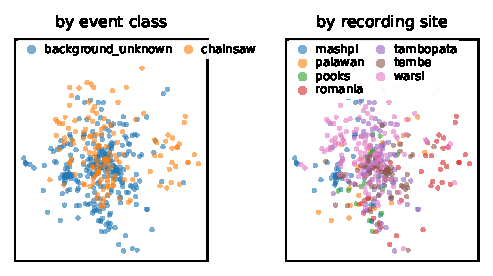
\includegraphics[width=\columnwidth]{figures/pca_cnn_threat_cnn_kaggle_augmented_v1.pdf}
\caption{PCA of the supervised-CNN embedding of held-out forest clips, colored by
event class (left) and by recording site (right). Structure tracks site at least
as strongly as class.}
\label{fig:pca}
\end{figure}

\paragraph{Takeaway.} Closed-set classifiers fail under site-level shift not
because they cannot discriminate threats, but because (i) their operating point,
calibrated on the source domain, does not transfer, and (ii) their representation
encodes site-specific structure. This motivates a detector whose decision
boundary is defined by the \emph{deployment site's own} background and whose
attribution is decoupled from a frozen, general-purpose representation, the
design of Section~\ref{sec:method}.
